\section{Visual Applications}
\label{sec:analysis}
The following examples illustrate how {\em Via} can help student,
instructor, and administrator stakeholders make sense of student data.

\subsection{Student Stakeholders}
\label{sec:student-stakeholders}

\begin{figure}
    \centering
    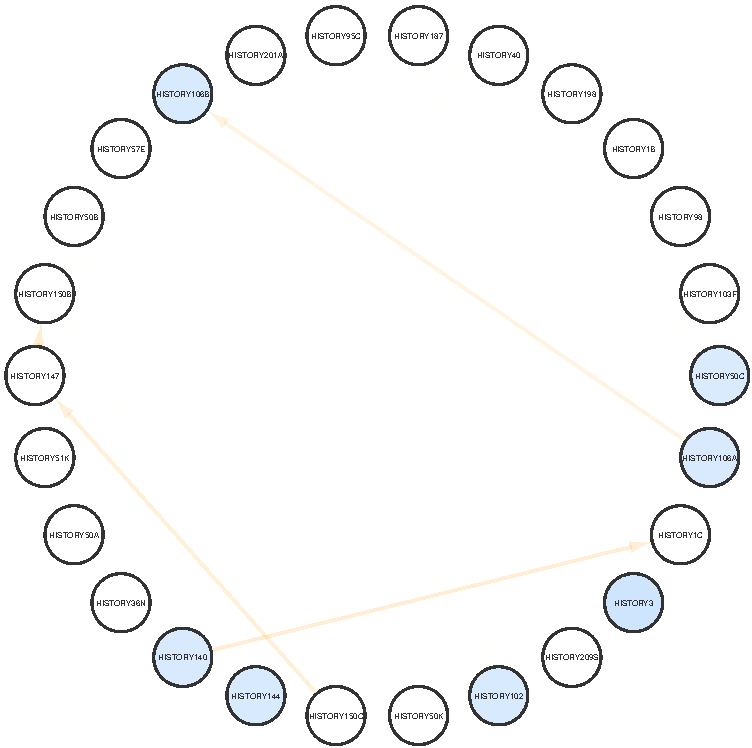
\includegraphics[width=0.55\columnwidth]{Figs/final-modularity-history.pdf}
    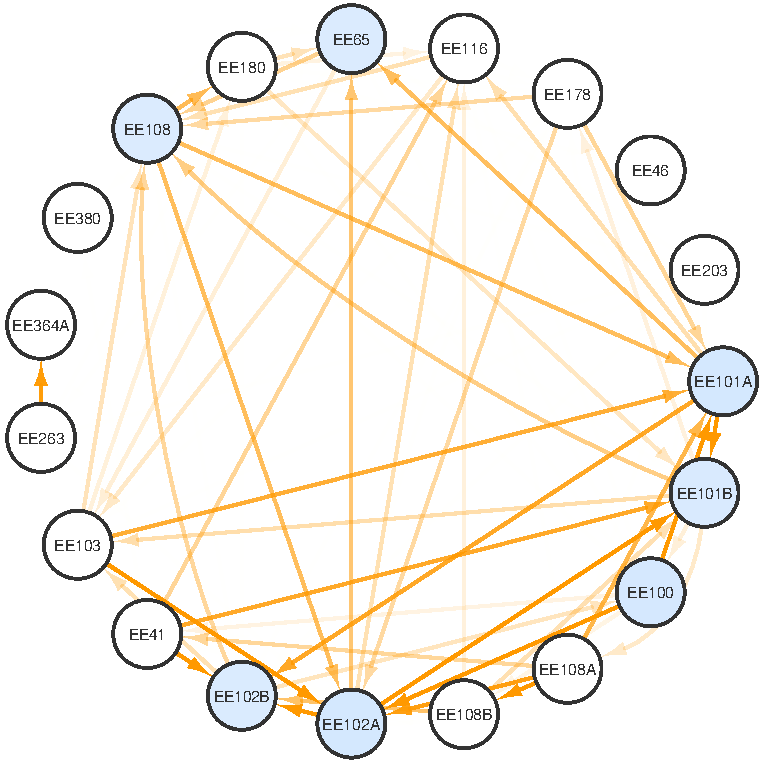
\includegraphics[width=0.44\columnwidth]{Figs/final-modularity-ee.pdf}
    \caption{A comparison between the student behavioral patterns in two departments---History (left) and Electrical Engineering (right)---from the years 2012-2016. Labels in the small circles are course names, such as ``\textsc{ee41}'' and ``\textsc{history198}''.}
    \label{fig:modularity}
\end{figure}

Departments differ by the degree to which requirements keep students
within the department. A department with fewer formal
intra-departmental requirements allows students to more easily sample
other areas of interest. Gaining an overview of such differences among
many departments is tedious. Prior student pathways tell the story
more directly.

In Figure~\ref{fig:modularity} we compare the interconnectivity of
the History and Electric Engineering majors, limited to course
enrollments of one academic year apart. The Electrical Engineering
department clearly has students take numerous internal courses as
indicated by the many orange links. History, in contrast, has students
take more outside courses. (Those outlinks are excluded from the
Figure.)

Note that this intra-cluster connectivity is equivalent to the graph
computational {\em modularity}. This metric represents the connectivity
of clusters within a graph, by calculating the over-representation of
edges among groups of nodes.

As a second use case, we illustrate how \textit{Via} can be leveraged
to discover ''try-me'' courses. Departments offer such service courses
for students majoring in unrelated fields, but who are interested in
exploring other areas of study. {\em Via} enables quick discovery of
such courses.

We find the ``try-me'' courses by creating a {\em Via} graph over
students of a single major. We then identify the most popular courses
within this generated graph that are not in that major. For instance,
by filtering on the History major, we observe that of the History
majors, nearly 28\% take \textsc{cs105}, and 21\% take
\textsc{cs106a}. These trends are visualized through variations in
node coloration in Figure~\ref{fig:history-try-me}.

\begin{figure}[h]
    \centering
    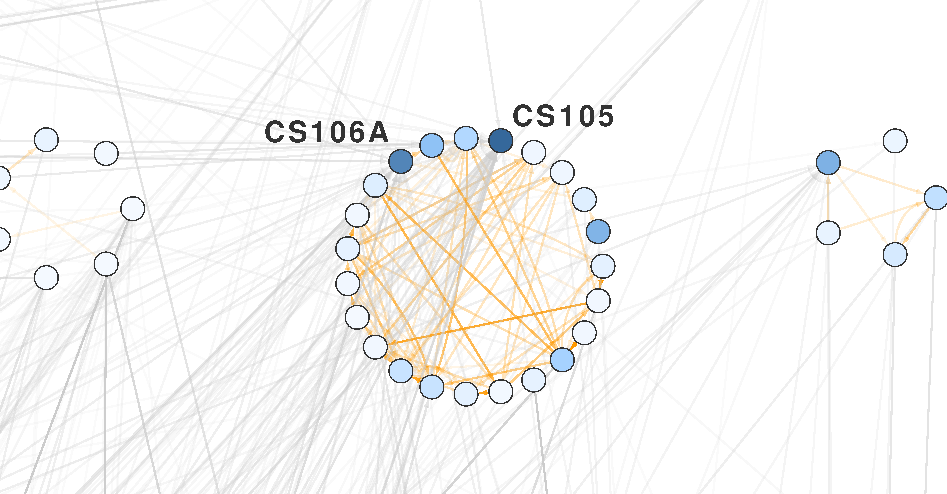
\includegraphics[width=.9\columnwidth]{Figs/final-history-try-me.pdf}
    \caption{A visualization of the most popular courses in the Computer Science department for History majors.}
    \label{fig:history-try-me}
\end{figure}

 Babad et al. have discovered that the primary reasons students decide
 to enroll in a particular course are the learning value of the class
 followed closely by the lecture style \cite{Babad2003}. Particularly
 difficult courses are avoided by students unless otherwise
 required. Our assessment of the recommended Computer Science
 ``try-me'' courses for History majors corroborates these
 results. Although \textsc{cs106a} is branded as the most enrolled
 introductory Computer Science course at the university from which we
 have acquired our dataset, \textsc{cs105} additionally presents
 itself as the Computer Science course for non-majors, and it is also
 known among students as less rigorous. Our \textit{Via} toolkit is
 thus able to offer a more personalized course discovery system for
 students of a particular major.
 
